% ICDE 2027 research track -- Experimental, Analysis, and Benchmark (EAB) paper.
% IEEE conference format: IEEEtran.cls V1.8b and IEEEtranN.bst are vendored here
% so the build does not depend on the local TeX distribution. The PVLDB-formatted
% version of this manuscript is the git tag `pvldb-manuscript` (decision D-015).
\documentclass[conference]{IEEEtran}
\usepackage{amsmath}
\usepackage{amssymb}
\usepackage{array}
\usepackage[numbers,sort&compress]{natbib}
\usepackage{booktabs}
\usepackage{graphicx}
\usepackage[hidelinks]{hyperref}
\hypersetup{
  pdftitle={[Experiment, Analysis, and Benchmark] Temporal Fields Are Not Temporal
    Correctness: Measuring Bitemporal and Deletion Semantics in Deployed Agent
    Memory},
  pdfauthor={Suan Lee},
  pdfsubject={ICDE 2027 Experiment, Analysis, and Benchmark paper},
  pdfkeywords={agent memory, bitemporal data, transaction time, data deletion,
    experimental analysis, benchmarking, reproducibility},
}

% Long typewriter identifiers do not hyphenate and push past the column edge.
% \allowbreak permits a break after a hyphen that is already there, rather than
% inventing one that would be misread as part of the identifier. Written out per
% identifier: a macro that walks the characters is easy to get subtly wrong, and
% an earlier attempt silently swallowed the hyphens it was meant to break after.
\newcommand{\embedmodel}{\texttt{text-\allowbreak embedding-\allowbreak 3-\allowbreak small}}
\newcommand{\runeseven}{\texttt{longmemeval-\allowbreak e7-\allowbreak v2}}
% Figure alt text is kept in the source for accessibility; IEEEtran has no
% mechanism to embed it, so the command is a no-op here.
\providecommand{\Description}[1]{}

% ICDE requires EAB titles to START with this tag; it is removed at camera-ready.
\title{[Experiment, Analysis, and Benchmark]\\
Temporal Fields Are Not Temporal Correctness:\\
Measuring Bitemporal and Deletion Semantics\\ in Deployed Agent Memory}

% ICDE review is single-blind: names and affiliations appear on the first page.
\author{\IEEEauthorblockN{Suan Lee}
\IEEEauthorblockA{School of Computer Science\\
Semyung University\\
Jecheon, South Korea\\
suanlee@semyung.ac.kr}}

\begin{document}


\maketitle

\begin{abstract}
Long-running agents accumulate facts that change, expire, and must sometimes be
deleted. Answering \emph{what was true then}, and \emph{what the agent knew then},
needs valid time and transaction time, and deletion must reach every store.
Agent memory systems advertise both; we ask where in their pipelines it holds.

We replay deterministic lifecycle histories, scored by an oracle that a second
implementation checks, into five open-source systems---Mem0, LangMem, Graphiti,
Cognee and Hindsight---and measure separately what a store retains, what its
retrieval selects for the asked time, what an answer asserts, and what deletion
removes. The later follow-up studies committed their predictions before they
ran; sixteen failed, and we report them. The layers disagree. Stores that
overwrite superseded values keep almost none of them and answer historical
questions only up to a ceiling the history fixes (Mem0: 0.364 against 0.385),
and Mem0 applies a correction about the past to the present. On the main grid, stores that keep
the history answer no valid-time question at their retrieval layer, yet one
common reader answers 0.73 to 0.77 of them from the same text where it carries
dates, and changing only the retention policy under a fixed retriever and
reader reproduces the split. Once a correction is stored, the systems' own
readers recover what was known before it far more often, by a strict count,
than retrieval or a common reader does. Three systems ignore prose deletion requests; native APIs, given the
right records, leave no purged value in our probes' answers but leave copies in
stores no query reads; and an unchecked search-and-delete caller erases up to
28 of 36 people it was never asked about.

We claim no novelty for bitemporal modelling or forgetting evaluation: the
contribution is a measurement contract and what it shows.
\end{abstract}

\begin{IEEEkeywords}
agent memory, bitemporal data, transaction time, data deletion,
experimental analysis, benchmarking, reproducibility
\end{IEEEkeywords}



\section{Introduction}

Agent memory must distinguish \emph{what was true at time $t$} (valid time)
from \emph{what the system knew then} (transaction time). Deletion must also
reach copies in history tables, vector stores and raw episode logs.

These needs are recognised. Graphiti attaches creation, validity, invalidity and
expiry timestamps to graph edges; Mem0 records add/update/delete history beside
a mutable vector store; Hindsight combines invalidation archives, histories,
audit logs and derived-record cleanup; and recent work makes the temporal model
explicit, from a graph-native bitemporal store to a bitemporal operator algebra
and a bi-temporal ledger with deterministic supersession.

We ask whether these representations produce correct temporal answers and
deletions. Retention, retrieval, answer synthesis and deletion can each succeed
while another fails; we measure them separately.

\paragraph{Contributions.}
(i) \emph{An evaluation contract} for agent memory (\S\ref{sec:setup}) that
separates what a store retains, what its retrieval selects for the asked time,
what an answer asserts and what a deletion leaves: one seeded history replayed
into every system and scored against an oracle; questions on both time axes,
asked at forward-replay checkpoints and of the final store; complementary
readings --- as returned, by one common reader, and by the value an answer
asserts, with the judge and annotators checked on answers of known verdict; and a deletion
protocol of prose requests, an oracle, an unchecked and a checked API caller,
and a store inventory. It reversed three of our own readings: a reader gap that
was answer wording, a purge category that asked less than its request, and
ceiling exceptions that were unapplied updates.
(ii) \emph{A controlled account of where temporal answers fail}. Changing only
the retention policy under a fixed retriever and reader reproduces the split we
see in the products (\S\ref{sec:reader}): overwriting stores answer historical
questions only up to a ceiling the history fixes, and their served memories
keep 0 and 7 of 75 superseded values (\S\ref{sec:bounds}); retaining stores
keep history but their retrieval layers do not filter it: the two that return
dates answer 0.73 to 1.00 when read, Graphiti's undated facts 0.11. The split
holds on a second backbone and in replicates; Mem0's current release changed
design (\S\ref{sec:releases}), so a classification belongs to a version's
observed behaviour, not to a product.
(iii) \emph{Version-bounded findings} on the measured releases: a consolidating
store applies a correction about the past to the present, and the systems' own
readers recover what was known before it far more often than retrieval or a
common reader (\S\ref{sec:corrections}); prose deletion is ignored by three
systems, native APIs leave no purged value in our probes' answers but leave
copies off the query path in three, and an unchecked search-and-delete caller
destroys unrelated data that a caller checking the name keeps
(\S\ref{sec:deletion}); LongMemEval's 62 supersessions show the same direction,
but no valid-time gold meets our two-model agreement criterion
(\S\ref{sec:realdata}); and reading, not writing, dominates the cost of the
one store with its own reader (\S\ref{sec:cost}).
Every number recomputes offline from sealed runs; code, data, sealed runs and
scripts are public at
\url{https://github.com/suanlab/temvera}.

\section{Related Work}

\paragraph{Both questions are database questions first.}
Valid time and transaction time are the two axes of temporal databases
\citep{snodgrass1985,jensen1999temporal}; TSQL2 \citep{snodgrass1995tsql2} formalised them in a query language,
and SQL:2011 standardised application-time and system-versioned tables
\citep{kulkarni2012sql2011}. TPC-BiH
\citep{kaufmann2013tpcbih} benchmarks time-travel queries on both axes over
relational engines. We take the semantics and the benchmarking stance from this
work: our oracle implements the same two axes, and our questions are the
agent-memory analogue of time-travel queries. Deletion has a database history
too. GDPR's right to erasure has been turned into database requirements and
benchmarked \citep{shastri2020gdpr}, argued for as a property to build in rather
than retrofit \citep{schwarzkopf2019gdpr}, and traced to conventional LSM storage, where
tombstones need not bound physical deletion latency
\citep{sarkar2020lethe}. Agent memory adds copies no database delete path knows
about --- extracted facts, LLM-written summaries, request logs --- and our
residue scan asks the same question of them.

\paragraph{Temporal modelling for agent memory is prior art.}
A graph-native bitemporal memory store \citep{graphnativebitemporal} keeps valid- and transaction-time
intervals with point-in-time retrieval, and TOKI \citep{toki} defines bitemporal operators
over a dual-row schema. MemStrata \citep{memstrata} pairs a bi-temporal ledger
with a deterministic (subject, relation, object) supersession rule and reports
stale-fact rate as its headline metric, and MemTX \citep{memtx} and MemTxn
\citep{memtxn} add transactional commit and recovery boundaries to agent memory.
We therefore claim none of these.

\paragraph{Forgetting evaluation is prior art.}
ForgetEval \citep{forgetevalpaper,forgeteval} generates seeded lifecycle cases
across supersession, decay, amnesia, purge and drift, calls each system's native
delete, and passes a case when no forbidden string reaches the top ten
retrieved; MemoryAgentBench \citep{memoryagentbench} evaluates selective
forgetting among four competencies. Springdrift \citep{springdrift} already
combines append-only memory, auditability and git-backed recovery. Bemula
\citep{bemula} sends forget requests in dialogue to six systems, scores leaks and
over-deletion from answers, and finds that none passes more than 1.5\% end to
end; MemCut \citep{memcut} recovers deleted secrets from objects that survive
its own deletion harness, and MemLeak \citep{memleak} from retained images and
correlated text. ForgetEval and Bemula judge deletion from retrieval or
answers. MemCut also snapshots surviving objects under its turn-anchored
deletion harness; our store inventory instead follows each measured library's
native deletion paths.

\paragraph{Measuring deployed memory.}
Zhou et al.\ \citep{agentnative} evaluate twelve memory systems on eleven
datasets from a data-management perspective, including update robustness on
LongMemEval's knowledge-update slice, cost and component ablations, and Wolff
and Bennati \citep{wolffcost} compare the accuracy and cost of Mem0, Graphiti and
Cognee. STALE \citep{stale} and StateMemBench \citep{statemembench} find that
memory systems often answer with a superseded state, Supersede \citep{supersede}
isolates that gap on LongMemEval's knowledge-update questions, and Ground Truth
First \citep{groundtruthfirst} asks as-of-date questions over facts with
validity intervals on its own backends, at replay checkpoints where valid and
transaction time coincide. These score the current state or valid time. Our comparison additionally
asks a fully ingested store what it \emph{knew} before a retroactive correction
and links this to deletion residue under the same lifecycle specification
(Table~\ref{tab:related}). They go further than we do elsewhere: Zhou et al.\ in
systems, data and cost, Bemula in forms of forgetting, attacks and backbones,
ForgetEval in failure categories.

\begin{table}[t]
\centering
\caption{What closely related studies evaluate, read from each work's full text
and, where released, its code (October 2026). \checkmark: evaluated; ---: not.
``Knew then'' asks what the system had recorded by an earlier time
(transaction time) as distinct from valid time; ``deletion residue'' reads a
deployed system's stores after a deletion, beyond what its answers expose.}
\label{tab:related}
\footnotesize
\setlength{\tabcolsep}{3pt}
\begin{tabular}{@{}lccccc@{}}
\toprule
Work & deployed & superseded & past & knew & deletion \\
 & systems & values & valid time & then & residue \\
\midrule
Zhou et al.\ \citep{agentnative}   & \checkmark & \checkmark & --- & --- & --- \\
STALE \citep{stale}                & \checkmark & \checkmark & --- & --- & --- \\
StateMemBench \citep{statemembench} & \checkmark & \checkmark & --- & --- & --- \\
Ground Truth First \citep{groundtruthfirst} & --- & \checkmark & \checkmark & --- & --- \\
ForgetEval \citep{forgetevalpaper} & \checkmark & \checkmark & --- & --- & --- \\
Bemula \citep{bemula}              & \checkmark & \checkmark & --- & --- & --- \\
MemCut \citep{memcut}              & \checkmark & --- & --- & --- & \checkmark \\
This paper                         & \checkmark & \checkmark & \checkmark & \checkmark & \checkmark \\
\bottomrule
\end{tabular}
\end{table}

\paragraph{Deployed systems and security.}
Mem0 \citep{mem0}, Zep/Graphiti \citep{zep,graphiti}, MemGPT/Letta \citep{memgpt},
HippoRAG~2 \citep{hipporag2} and Hindsight \citep{hindsight} form the baseline landscape. MINJA \citep{minja} shows query-only poisoning; MemLineage \citep{memlineage}
proposes lineage-based action gating; A-MemGuard \citep{amemguard} is a current
defence baseline.

\paragraph{What is left.}
No prior work we found measures, under one controlled history, both bitemporal
answer correctness \emph{and} where deleted content physically survives across a
system's derived stores; the works above each measure one side, on other
systems or by other means. Our literature review is single-reviewer with a
deterministic 10\% rescreen; searches, exclusions and rescreens are logged and
frozen with the artifact, the last search on 19 October 2026, and the seven
closest works were re-read in full, with their released code, on 23 October.

\section{Which fragment of bitemporal semantics does each system implement?}
\label{sec:fragment}

The query we need is standard \citep{snodgrass1985}: for subject $s$ and
attribute $a$, return the value valid at event time $V$ according to what the
store had recorded by transaction time $T$. Our query and deletion contract
examines six capabilities, and the systems differ less in whether they \emph{have} temporal
metadata than in what can be \emph{predicated} on it. We therefore classify
support into five levels, which account for what we measure in
\S\ref{sec:results}:

\begin{description}[\IEEEsetlabelwidth{\textsc{mismatch}}]
  \item[\textsc{absent}] the information is not stored;
  \item[\textsc{prose}] stored, but only inside free text, so no predicate can
        filter on it;
  \item[\textsc{off}] a queryable field exists and a filter is available, but is
        not applied by the default retrieval path;
  \item[\textsc{mismatch}] a queryable field exists and is applied, but denotes a
        different timeline than the query requires;
  \item[\textsc{yes}] representable, queryable, and applied.
\end{description}

\begin{table}[t]
\centering
\caption{Support for six capabilities of the query and deletion contract.
Levels are defined above. Entries are what we observed in the shipped versions,
not what documentation claims.}
\label{tab:fragment}
\footnotesize
\setlength{\tabcolsep}{3.5pt}
\begin{tabular}{@{}lcccc@{}}
\toprule
Capability & Ref.\ impl. & Mem0 & LangMem & Graphiti \\
\midrule
C1 valid-time interval    & \textsc{yes} & \textsc{absent} & \textsc{prose} & \textsc{yes} \\
C2 transaction time       & \textsc{yes} & \textsc{absent} & \textsc{absent} & \textsc{mismatch} \\
C3 supersession closes    & \textsc{yes} & overwrite & overwrite & partial \\
C4 valid-time predicate   & \textsc{yes} & --- & --- & \textsc{off} \\
C5 as-of predicate        & \textsc{yes} & --- & --- & \textsc{absent} \\
C6 clears serving stores & partial & \textsc{yes} & \textsc{yes} & partial \\
\bottomrule
\end{tabular}
\end{table}

C6 concerns the inspected serving stores, not backups: the reference purge
leaves earlier values under the request's scope, and Graphiti retains queryable
node summaries (\S\ref{sec:deletion}). Three entries carry most of the
explanatory weight.

\textbf{C2 \textsc{mismatch} is a second timeline, not a bug.} Two recording
times must be told apart. The \emph{physical} one is when the store wrote a
fact; the \emph{logical} one is when the agent learned it --- the date of the
conversation turn that stated it. In live use they coincide. They part whenever
a history is imported, backfilled, replayed or ingested late, and an agent's
``what did I know on 18 February'' asks about the logical one. Graphiti's
\texttt{created\_at} and \texttt{expired\_at} are a correct physical
transaction time: in our runs they carry 2026 timestamps for turns dated 2025.
Graphiti has no field for the logical time, so no predicate over its store can
express ``as of what was known on 2025-02-18'' for any history not ingested
live. This is why we ask transaction-time questions in two ways: at each
checkpoint of a forward replay, which restricts every store to earlier inputs,
and of the final store after the whole history (\S\ref{sec:corrections}), which
needs either a transaction-time predicate, which none of them has, or a reader
over source text that carries its recording dates --- and why C5 is \textsc{absent} rather
than \textsc{off}.

\textbf{C1 \textsc{prose} is the distinction a capability checklist misses.}
LangMem does retain validity information --- its stored memories contain strings
such as ``valid from January 3, 2025''. But the store holds opaque values under
a namespace, so validity is legible to a reader and invisible to a query
planner. A survey that asked ``does the system record when a fact became true''
would score LangMem as supporting valid time; no predicate can use it.

\textbf{C3 separates closing an interval from overwriting a row.} Mem0 and
LangMem consolidate: a superseding fact replaces its predecessor, so the prior
value is destroyed rather than bounded. We read whole stores to check this,
not top-five retrievals: after ingesting each of the ten revision-only histories
of the main grid, Mem0's served memories (its \texttt{get\_all}; the history
table no query reads is not counted) hold none of 75 superseded values and
LangMem's store holds 7, while Graphiti's holds all 75. Graphiti closes intervals by setting
\texttt{invalid\_at}, but not reliably: for 61 of the 75 some edge stating the
value has the field set, and for 43 it is the day the successor took effect. (An
earlier inspection that also found self-contradictory intervals ran on a graph
later withdrawn for contamination, \S\ref{sec:negative}; we no longer rely on
it.) C3 is therefore the axis on which the two design families separate, and
\S\ref{sec:results} measures the consequence: consolidating stores lose
history, while Graphiti retains it and does not filter it.

C1 and C2 are data-model properties; C3 is filled by the LLM extraction step,
so in LLM-backed temporal stores the extractor, not the schema, decides what the
temporal fields hold. The table covers the three systems whose stores we
inspected; Cognee and Hindsight are characterised by measured behaviour
(\S\ref{sec:reader}).

\subsection{What the systems say they do}
\label{sec:claims}

Table~\ref{tab:claims} compares packaged documentation with measurements,
quoting the distribution's \texttt{METADATA}.

\begin{table}[t]
\centering
\caption{Documented temporal claim against measured \texttt{valid\_time}: exact at
the retrieval layer, and read by the common reader of \S\ref{sec:reader}. Quotes are verbatim from the distribution's own
\texttt{METADATA} at the version measured.
Claim text and checksums are archived with the artifact.}
\label{tab:claims}
\small
\begin{tabular}{@{}l>{\raggedright\arraybackslash}p{3.7cm}cc@{}}
\toprule
System & Documented temporal claim & exact & read \\
\midrule
Graphiti  & ``Query what's true now, or what was true at any point in time'' & 0.000 & 0.113 \\
Hindsight & ``Temporal + Semantic + Entity Memory Architecture'' & 0.000 & 0.769 \\
Cognee    & none; documents a \texttt{forget} operation & 0.000 & 0.728 \\
Mem0      & none; ``long-term memory'' & 0.364 & 0.374 \\
LangMem   & none; ``extracts, consolidates'' & 0.323 & 0.364 \\
\bottomrule
\end{tabular}
\end{table}

The ordering inverts at the retrieval layer: the two systems that advertise
temporal capability answer no valid-time question there, while the two that
advertise none score highest. Read by an LLM the advertised systems do recover
the history (\S\ref{sec:reader}), so their claims are not false, but the
retrieval path a caller uses does not deliver them; documentation is no guide to
which layer answers. Mem0 and LangMem make no temporal promise, so their low
scores are a design consequence, not a discrepancy.

\section{Experimental Setup}\label{sec:setup}

\paragraph{Workload.} A seeded generator emits typed histories over
entity/attribute state machines with configurable reconfirm, expire and purge
probabilities. Query truth is computed by the oracle independently of retrieval.

\paragraph{Why synthetic histories first.} Exact answers on both time axes need
a history in which every valid interval and every recording time is known, and
whose mix of revision, expiry and purge can be varied. The knowledge-update
slice of LongMemEval supplies current-value gold, not both time axes. Synthetic
histories give that control; benchmark conversations test transfer under an
explicit persistence assumption (\S\ref{sec:realdata}).
The price is realism, which is why that check is read as direction, not as
rates.

\paragraph{Rendering.} Histories are rendered to dated conversational turns.
The generator's synthetic tokens (\texttt{entity-000}, \texttt{place-38})
collapse under a semantic embedder, leaving systems unable to tell entities
apart, so an injective relabelling maps them to distinct natural names. The
relabelling preserves oracle semantics exactly and doubled Mem0's measured exact
accuracy, isolating tokenisation from temporal semantics.

\paragraph{Replay.} Transaction time is monotonic, so turns are ingested in
recorded order and every query is answered at the checkpoint matching its
transaction time. This supplies the store's earlier input state without a
transaction-time predicate; it does not guarantee a correct answer. Whether a store
that has seen everything can still say what it knew earlier is a different
question, which \S\ref{sec:corrections} asks of the final store.

\paragraph{Scoring.} Deterministic. Let $E$ be the expected values at the queried
$(\text{valid time}, \text{transaction time})$ and $S$ the superseded values for
the same subject/attribute. A response is \emph{exact} iff every $e \in E$ occurs
in the returned text and no $s \in S$ does; when $E = \emptyset$ (the fact was
purged or expired) exactness requires that no $s \in S$ occurs. This tests
known-value absence, not semantic abstention: an unrelated answer can pass.
The scorer does not interpret negation. Evidence recall is $|E \cap \text{returned}| / |E|$ for nonempty $E$
(and the absence indicator otherwise), and stale-use is
the fraction of returned values drawn from $S$. \textbf{Because exactness
quantifies over the whole returned set, it is a function of the retrieval budget
$k$}; we set $k{=}5$ throughout and report a sweep over $k$ in
Figure~\ref{fig:budget}. Rates are case-weighted with Wilson 95\% intervals, and
abstention is computed only over cells that contain abstention cases. Two
comparisons are cell-averaged instead, because they aggregate cells whose
denominators differ --- the internal baselines of \S\ref{sec:results} and
the filtered-Graphiti runs --- and both are marked where they are used.
Cases share the histories they are asked of, so inference is made over
histories, not cases: the 484 questions come from 20 histories generated from 5
seeds. For each comparison the conclusions rest on --- a family of six, declared
in the artifact before this analysis --- the paired difference has the same sign
in all 20 histories and all 5 seeds, and an exact sign-flip permutation test over
histories gives $p = 1.9 \times 10^{-6}$, the smallest it can; clustered by seed
the test cannot go below $0.0625$, which is what it gives. Intervals resample
whole histories (4{,}000 draws) and collapse to a point where every history
agrees, which is not certainty about other histories. The raw reader comparison
in the family is one of answer form (\S\ref{sec:reader}). The one pair we call
close --- Mem0 against Graphiti at $k{=}1$ --- is equivalent within 0.10
(difference $+0.026$, 90\% cluster interval $[0.000, 0.057]$) but not within
0.05, so we do not call the two the same.

\paragraph{The oracle defines ground truth.} Expected values come from our
reference implementation, a typed append-only event log (\texttt{ingest},
\texttt{reconfirm}, \texttt{supersede}, \texttt{expire}, \texttt{purge}) folded
into beliefs that carry a valid-time interval and a transaction time. A second
SQLite implementation of the same specification checks that fold; the two agree,
which is a differential test of our own code, not external validation. The
reference implementation is not a system under test: it scores $1.0$ by
construction, appears only as a scale anchor and as the reference column of the
deletion scan, and its other machinery plays no part in the measurements.

\paragraph{Systems.} Internal baselines (append-only, full/recent context, BM25,
last-write-wins) and the oracle, and five external systems run at their
libraries' defaults, as a user would deploy them (Table~\ref{tab:settings}).
All use \texttt{gpt-4o-mini} (\texttt{gpt-4o} only where \S\ref{sec:results}
says so). The Hindsight runs did not record their version, but the daemon that
served them, started once before them, applied the 96 schema migrations of
\texttt{hindsight-api 0.9.1} and of no other release, so they ran 0.9.1. LangMem and
Cognee require \texttt{openai} major versions incompatible with the pinned Mem0
and Graphiti, so they run in isolated interpreters behind a stdio protocol. Runs
are sealed with canonical config, environment, source hash and per-file
checksums.

\begin{table}[t]
\centering
\caption{Settings of the measured systems. Temperatures are for extraction and,
where an LLM writes the answer, reading; ``default'' leaves the provider's own.
Embeddings are \embedmodel{} except Hindsight's local
\texttt{BAAI/bge-small-en-v1.5}.}
\label{tab:settings}
\footnotesize
\setlength{\tabcolsep}{2.5pt}
\begin{tabular}{@{}l>{\raggedright\arraybackslash}p{2.25cm}l>{\raggedright\arraybackslash}p{2.45cm}@{}}
\toprule
System & Store & Temp. & What is scored \\
\midrule
Mem0 0.1.118      & Qdrant + SQLite history     & 0 & top-5 memories \\
LangMem 0.0.30    & LangGraph in-memory         & default & top-5 memories \\
Graphiti 0.29.2   & Neo4j 5.26                  & 0 & top-5 facts (hybrid RRF) \\
Cognee 1.4.2      & SQLite, LanceDB, graph DB   & 0 / 0 & top-5 chunks; or its reader \\
Hindsight 0.9.1   & embedded PostgreSQL         & 0.1 / 0.9 & recall (budget ``mid''); or its reader \\
\bottomrule
\end{tabular}
\end{table}

\paragraph{Versions.} Our claims are about the versions named above, measured
between July and October 2026; every sealed run records its environment, and
\S\ref{sec:releases} re-runs the releases current on 22 October 2026. What we
conclude concerns observed behaviour --- whether a version overwrites or
retains, and where filtering happens --- not a product name.

\section{Results}\label{sec:results}

\subsection{The oracle is exact; non-temporal baselines are not}

Across 270 cells (3 profiles $\times$ 3 scales $\times$ 3 revision counts, 10 seeds
each) the oracle held exact, recall and stale-use at $1/1/0$, so the rendering
and the scorer round-trip the intended semantics. Baselines that ignore time do
not: returning the whole history recalls the evidence ($0.915$) but answers
$0.272$ exactly, $0.255$ under high churn with $0.662$ stale-use;
last-write-wins answers $0.603$ and the most recent turn $0.576$
(cell-averaged; the full table is in the artifact). They are strawmen that show
the harness discriminates, not competitors.

\subsection{Two designs: consolidate, or retain without filtering}

This subsection examines three systems in depth; \S\ref{sec:reader} adds two
more. All run the \textbf{same 20-cell grid by design} (5 seeds $\times$ 2
scales $\times$ 2 profiles, 484 cases per system), with Graphiti under the hybrid
retrieval it actually ships and Mem0 with a per-run isolated history database; we report case-weighted
(micro) rates with denominators and Wilson 95\% intervals, since several
categories rest on few cases.

\begin{table}[t]
\centering
\caption{Exact accuracy by lifecycle category over the matched 20-cell grid, 484
cases per system. LangMem is included because a two-system taxonomy cannot be
evidence for itself. Rates are case-weighted; Wilson 95\% intervals are shown where
the denominator is small. \texttt{purge} and the overall rates use the
request's own scope, under which nothing of the purged attribute may be
answered (\S\ref{sec:deletion}); as our generator first specified it, purge
reads 0.044, 0.133, 0.022 and overall 0.603, 0.576, 0.196. Evidence recall (expected
values an answer contains; for a question expecting none, naming no superseded
value) and stale-use (named values that are superseded) are cell-averaged as
sealed, purge as first specified. The oracle is $1.0$ by construction.}
\label{tab:external}
\begin{tabular}{lccc}
\toprule
Category & Mem0 & LangMem & Graphiti \\
\midrule
\texttt{transaction\_as\_of} & 0.952 & 0.890 & 0.412 \\
\texttt{valid\_time}         & 0.364 & 0.323 & 0.000 \scriptsize{[.00,.02]} \\
\texttt{expiry\_boundary}    & 0.125 \scriptsize{(2/16)} & 0.438 \scriptsize{(7/16)} & 0.000 \scriptsize{(0/16)} \\
\texttt{purge}               & 0.000 & 0.200 & 0.000 \\
\midrule
Overall exact                & 0.599 & 0.583 & 0.194 \\
Evidence recall (macro)      & 0.666 & 0.647 & 0.937 \\
Stale-use (macro)            & 0.356 & 0.343 & 0.528 \\
Exact at $k{=}1$             & 0.626 & 0.601 & 0.450 \\
\bottomrule
\end{tabular}
\end{table}

\begin{figure}[t]
\centering
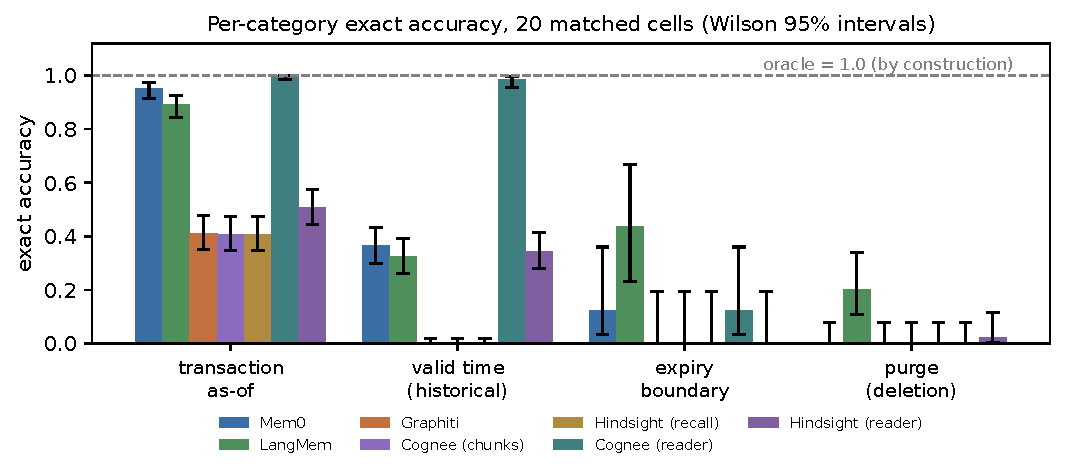
\includegraphics[width=\linewidth]{figures/categories.pdf}
\Description{Grouped bar chart of exact accuracy by lifecycle category for all seven configurations. Mem0 and LangMem are high on transaction-scoped queries and moderate on valid time; the three retrieval-layer retaining stores are near zero on valid time; Cognee's reader is near one on transaction and valid time. Error bars are widest on expiry, which rests on sixteen cases.}
\caption{Per-category exact accuracy over the matched cells, all seven
configurations. Expiry rests on 16 cases per system, so even a score of zero
admits accuracies up to $0.19$; we draw no conclusion from that category.}
\label{fig:categories}
\end{figure}

\textbf{Two systems consolidate; one retains without filtering.} LangMem was
added precisely because a typology drawn from the same two systems it describes
is not evidence. It lands in the Mem0 class on every axis --- exact $0.583$,
recall $0.647$, stale-use $0.343$, high \texttt{transaction\_as\_of} ($0.890$)
against low \texttt{valid\_time} ($0.323$), and budget-stability ($0.601 \to
0.583$) --- despite an independent implementation and no database server. It is
not uniformly weaker: it handles expiry better than either ($0.438$ against
$0.125$ and $0.000$), so the consolidation signature is specific rather than
general weakness.

\textbf{Mem0 consolidates.} It is strong on transaction-scoped current queries
($0.952$) and much weaker on historical valid time ($0.364$). Of its non-exact
cases, 87.6\% (170/194) return a stale or deleted value with the expected value
\emph{absent} --- absence from these answers; the separate census supports loss from the
served store ---
and this is stable across retrieval budgets (Figure~\ref{fig:budget}).

\textbf{Graphiti retains but does not filter.} It reaches $0.937$ evidence
recall and returns an item naming the queried subject at rank~1 in 91.3\%
(442/484) of cases, yet scores $0.194$ exact, because it returns superseded
revisions alongside the current one. \textbf{This deficit is budget-dependent,
and we report it as such}: our scorer requires every expected value and no
superseded value across the returned set, so a system that returns $k$ facts
about a one-attribute subject is penalised for its own retained history. At
$k{=}1$ the two systems' valid-time accuracy is close ($0.379$ against $0.354$;
paired difference within 0.10, not shown within 0.05, \S\ref{sec:setup}); as $k$ grows Graphiti collapses to $0.000$ while Mem0 is
nearly flat (Figure~\ref{fig:budget}). We therefore do not claim Graphiti cannot represent
valid time. The defensible claim is narrower and does not depend on $k$: its
retrieval does not apply the validity metadata it stores, so downstream filtering
is left to the caller.

\begin{figure}[t]
\centering
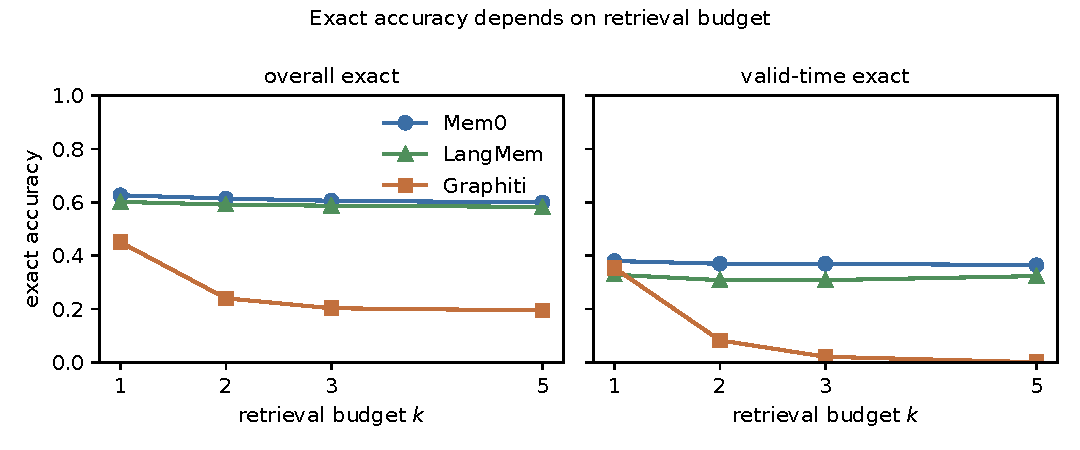
\includegraphics[width=\linewidth]{figures/budget.pdf}
\Description{Line chart of exact accuracy against retrieval budget k from one to five. Mem0 and LangMem are nearly flat across budgets; Graphiti starts close to them at k equals one and falls steeply as k grows, reaching zero on valid time at k equals five.}
\caption{Exact accuracy versus retrieval budget $k$ on matched cells. The
all-or-nothing conjunct in our scorer makes Graphiti's measured deficit grow
with $k$; at $k{=}1$ the two systems are close on valid time. Purge and overall
use the request's own scope. Budget
must be reported for any metric of this shape.}
\label{fig:budget}
\end{figure}

\textbf{Two fairness objections, tested.} Earlier runs disabled Graphiti's BM25
channel --- a workaround for a bug in an embedded backend we did not use --- and
ran Mem0 against a shared history database that its own library corrupts under
contention. We re-ran both under corrected configurations. Neither changed the
result: on the six cells both runs share, Graphiti under its shipped hybrid
retrieval answers 29 of 154 against 28 cosine-only, with 0 of 44 valid-time
questions either way, and Mem0 with an isolated database scores $0.599$ against
$0.616$. These reruns were also our
first same-protocol replication, and it is instructive: Mem0's expiry accuracy
moved $0.000 \to 0.125$ (2 of 16 cases) between runs, exactly the instability its
Wilson interval predicts. We therefore draw no conclusion from either system's
expiry number.

\textbf{A stronger backbone moves no system across the divide.} Re-running the
whole 20-cell grid with \texttt{gpt-4o} in place of \texttt{gpt-4o-mini},
otherwise unchanged, moves no category of Mem0 or Graphiti by more than 2 of its
cases. Mem0 goes from $0.599$ to $0.603$ overall and from $0.364$ to $0.374$ on
valid time; Graphiti from $0.194$ to $0.192$ overall, and on valid time it
answers 0 of 195 under both. The other three move more but stay on their side:
LangMem's valid-time accuracy falls from 0.323 to 0.262, still under the ceiling
of \S\ref{sec:bounds} with no answer above it, and its transaction-scoped
accuracy from 0.890 to 0.789, below the 0.80 we had predicted; Hindsight's
retrieval layer answers 0 of 195 valid-time questions under both; Cognee's
reader answers 194, Hindsight's 159 exactly where it answered 67. The exact gap
between the two readers therefore depends on how the model words its answers,
which \S\ref{sec:reader} shows directly; the design classes do not.

\textbf{Repeated runs agree, except one reader.} Three further runs of every
configuration on four of the grid's cells (97 cases), otherwise identical,
reproduce the cited overall accuracy exactly for Mem0 and Graphiti (58 and 19),
for Cognee's reader (84) and for the retrieval layers of Cognee and Hindsight
(19), move LangMem by at most 1 case, and leave every retaining retrieval layer
at 0 of 38 valid-time questions. Hindsight's reader, which reads at temperature 0.9, moves
by up to 10 cases and answers 8, 12 and 14 valid-time questions where the cited
run answered 19, though still fewer than Cognee's reader (38) in every run.
Run-to-run variation is below the effects we report everywhere except in that
reader's exact score, which we therefore do not read as a stable number.

\textbf{Does Graphiti's own filter repair it?} Enabling its native valid-time
\texttt{SearchFilter} raises exact from $0.224$ to $0.318$ and cuts stale-use
from $0.561$ to $0.360$, but collapses evidence recall from $0.873$ to $0.318$:
precision is bought by discarding evidence, and valid-time remains $0.093$.
(Rates in this paragraph are cell-averaged, matching how the filtered runs were
scored; the case-weighted valid-time is $0.114$.)
Two structural limits cap it. First, the filter's predicate is only as good as
the extracted \texttt{invalid\_at} it reads: in the clean full-store census of
\S\ref{sec:fragment}, 14 of 75 superseded values have no invalidated edge at
all, so a stale edge satisfies \texttt{invalid\_at IS NULL} at every event time
and is returned regardless. Second, \texttt{created\_at}/\texttt{expired\_at}
record physical ingestion, not the logical recording time of a replayed
history, so no \texttt{as-of} bound on the logical axis is expressible. With
\texttt{gpt-4o} in place of \texttt{gpt-4o-mini} on four matched cells, filtered
valid-time is unchanged ($0.111 \to 0.111$) while \texttt{transaction\_as\_of}
improves ($0.514 \to 0.625$); with two seeds we draw no conclusion about the
extractor's share from either.

\subsection{Deletion: with the right handles the API passes our probes; prose mostly does not}
\label{sec:deletion}

We ran all five systems through one deletion protocol, with its predictions
committed before the runs. Ten seeded histories hold 24 people whose attribute
is purged and 36 who are never purged. Each system ingests a history, including
the request, in one of three wordings, none of which restates the value
(``Permanently delete everything you recorded about $X$'s $A$'', ``Please forget
$X$'s $A$; I do not want it kept'', ``$X$ has asked for their $A$ to be erased
from your memory''). Two further conditions add the native API after the first
wording: an \emph{oracle} caller deletes every unit whose stored text holds a
value the person ever had, the most any caller could do; an \emph{unchecked}
search-and-delete caller, which does not know the value, asks the store about
$X$'s $A$ and deletes whatever comes back. We then ask every person's attribute and record a leak if
any value it ever had appears in the answer, read every store we inventoried
through its own library (the inventory is in the artifact), and count the never-purged people whose current value is gone
(Table~\ref{tab:deletion}).

\begin{table}[t]
\centering
\caption{Deletion in five systems over ten histories: purged people (of 24)
whose value still appears in the answer, by condition; never-purged people (of
36) still answered after the unchecked and the name-checked caller's deletions;
histories (of 9 with a purge) in which a store no query reads still holds a
purged value after the oracle's deletions.}
\label{tab:deletion}
\footnotesize
\setlength{\tabcolsep}{2.6pt}
\begin{tabular}{@{}lcccccccc@{}}
\toprule
 & \multicolumn{3}{c}{prose wording} & \multicolumn{2}{c}{API caller} & \multicolumn{2}{c}{kept} & off-path \\
System & 1 & 2 & 3 & oracle & uncheck. & uncheck. & checked & residue \\
\midrule
Mem0      & 24 & 2  & 24 & 0 & 0 & 8  & 36 & 9 \\
LangMem   & 15 & 3  & 6  & 0 & 0 & 19 & 33 & 0 \\
Graphiti  & 24 & 24 & 24 & 0 & 0 & 18 & 36 & 0 \\
Cognee    & 24 & 24 & 24 & 0 & 0 & 33 & 36 & 9 \\
Hindsight & 24 & 24 & 24 & 0 & 0 & 36 & 36 & 9 \\
\bottomrule
\end{tabular}
\end{table}

\textbf{Prose is ignored by three systems, and by two only sometimes.} Graphiti,
Cognee and Hindsight leak every purged person under every wording. Mem0 depends
on the words: told ``Please forget'', its extractor emitted 23 \texttt{DELETE}
actions and 2 people leak; told the other two, 24 of 24 leak, and it logged no
dropped action in any of these runs, so the failure is not the defect of
\S\ref{sec:external}. LangMem leaks 15, 3 and 6: its memory manager ships with
deletion disabled, so it rewrites memories instead, and loses never-purged
people on the way (it answers 30 of 36 under the first wording). With deletion
enabled it leaks none under any wording, but keeps only 6, 8 and 2 of the 36
people it was never asked about: its manager deletes far more than it is told. We had
predicted that every system would leak at least 80\% under every wording; that
holds for three systems and fails for Mem0 and LangMem.

\textbf{With the right handles, no API leaves a purged value in our probe's
answers, and something survives elsewhere.} Under the oracle caller no purged person leaks in
any system. A store no query reads still holds the value in all 9 histories for
Mem0 (its history table), Cognee (its relational database) and Hindsight (its
log of LLM requests). Graphiti's entity summaries, which \texttt{remove\_episode}
does not rewrite, hold it in all 9 as well; they are text a node search could
return, though our probe did not surface them. Cognee's \texttt{forget} leaves it
in its graph or vector store in up to 3 histories. Only LangMem, whose single
store is the one it serves from, keeps nothing.

\textbf{Without the handles, an unchecked caller deletes other people's data;
a checked one does not.} The unchecked caller also removes every purged value,
but a search for one person returns other people's memories, and it deletes them
too. Of the 36 never-purged people, Mem0 still answers 8, Graphiti 18, LangMem
19, Cognee 33 and Hindsight 36. A caller that deletes only the returned units
naming the person removes every purged value as well and keeps all 36 in Mem0,
Graphiti, Cognee and Hindsight, and 33 in LangMem (30 under the oracle caller;
these are separately ingested stores, so the gap is not the caller's). The over-deletion is the caller's, not the API's granularity, but only
because in these histories one unit holds one person's statement; units that
mix people or attributes are untested.

\textbf{Deletion and past-time questions need one semantics.} After a purge,
what should ``What was $X$'s home city in January?'' return? Erasure can be a
valid-time event (the fact stops being true), a transaction-time event (the
system stops having known it) or the physical removal of both, and the answer
differs for each. None of the five systems states which it implements, and our
own generator did not either: its typed purge removed only the latest value
while the request asked for everything, so our reference implementation still
holds earlier values in the projections a query reads, and 29 of the grid's 45
purge questions expected a value the request had asked to delete
(\S\ref{sec:reader}). We report both readings and use the request's own scope
here.

\textbf{The API requires caller-side selection.} The API surface locates the
record-selection responsibility; it does not by itself explain whether an
extractor acts on a prose request.
We inspected the installed distributions rather than their documentation:

\begin{table}[t]
\centering
\caption{Finest unit each deletion API can name, read from the distribution.
None of these low-level calls accepts a subject--attribute content predicate;
a caller must resolve the request to record handles.}
\label{tab:deletion-api}
\small
\begin{tabular}{@{}l>{\raggedright\arraybackslash}p{4.6cm}@{}}
\toprule
System & Finest nameable unit \\
\midrule
Mem0      & one memory id (\texttt{delete}), or a whole user/agent/run scope \\
Graphiti  & one episode, i.e.\ one ingested turn \\
Cognee    & one data item (\texttt{forget}; \texttt{delete} is soft by default), one dataset, or everything the user owns \\
LangMem   & one memory key; its memory manager's own deletions ship disabled (\texttt{enable\_deletes=False}) \\
Hindsight & one document (one retained input), or the whole bank \\
\bottomrule
\end{tabular}
\end{table}

These APIs require the caller to map a subject and attribute to record
handles. Cognee's documented \texttt{forget}, for example, takes a
\texttt{data\_id}, a dataset or \texttt{everything}; the caller must first
identify the items holding the fact. Selection and deletion are distinct
responsibilities, just as retention and filtering are.

\subsection{Is the information lost, or merely unfiltered?}
\label{sec:reader}

Cognee isolates reading from retention: it stages text, builds a graph, and
answers either by
returning retrieved passages (\textsc{chunks}) or by having an LLM answer over
the graph (\textsc{graph-completion}, its default). Both configurations run the
same 20-cell grid as the other systems (484 cases each):

\begin{table}[t]
\centering
\caption{Five systems, and two of them read both ways. ``Exact'' is the grid's
scorer on what the configuration returned. Each retrieval-layer row is also read
by one common reader over its top five (\texttt{gpt-4o-mini}, temperature 0);
each reader row is credited instead with the value its own answer asserts, by an
asserted-value judge. The two procedures differ and are not compared with each
other. Hindsight's retrieval budget is qualitative and cannot be set to the $k$
used elsewhere. \texttt{purge} and overall use the request's own scope.}
\label{tab:reader}
\footnotesize
\setlength{\tabcolsep}{2.4pt}
\begin{tabular}{@{}lccccc@{}}
\toprule
 & & \multicolumn{3}{c}{\texttt{valid\_time}} & \\
Configuration & overall & exact & common & judged & \texttt{purge} \\
\midrule
Mem0 (consolidates)              & 0.599 & 0.364 & 0.374 & --- & 0.000 \\
LangMem (consolidates)           & 0.583 & 0.323 & 0.364 & --- & 0.200 \\
Graphiti (retains)               & 0.194 & 0.000 & 0.113 & --- & 0.000 \\
Cognee \textsc{chunks} (retains) & 0.192 & 0.000 & 0.728 & --- & 0.000 \\
Hindsight \textsc{recall} (retains) & 0.192 & 0.000 & 0.769 & --- & 0.000 \\
\midrule
Cognee \textsc{graph-completion} & \textbf{0.872} & \textbf{0.985} & --- & 1.000 & 0.000 \\
Hindsight \textsc{reflect}       & 0.380 & 0.344 & --- & 1.000 & 0.022 \\
\bottomrule
\end{tabular}
\end{table}

\textbf{The retrieval layer fails uniformly.} Three independently built
retaining systems land within noise of each other --- Graphiti $0.194$, Cognee
$0.192$, Hindsight $0.192$ overall, and all three score $0.000$ on valid time
over 195 cases each. Retaining history without filtering it is shared by all
three retaining systems we measured, not a quirk of one implementation.

\textbf{Read, the retaining stores recover most of it.} Two readings, each
fixed and preregistered before it was run, separate what a store holds from how
its answers are worded. A common reader --- one prompt at temperature 0 over
each store's top five --- answers 142 and 150 of 195 valid-time questions from
Cognee's chunks and Hindsight's recall, which the same text unread answers 0 of;
we had predicted at least 0.80, and both fall short. From Graphiti's facts, which
mostly carry no dates, it answers 22. The systems' own readers do better.
Cognee's answers 192 exactly. Hindsight's answers only 67 exactly, but names
the right value in all 195 and then the later one, which the exact scorer
counts as wrong. An asserted-value judge
--- which agrees with the exact scorer on 1{,}202 of the 1{,}203 answers that scorer
accepts, and with a second judge on 99.6\% of all of them, and is right on 279
of 280 answers whose verdict we fixed by construction (seven templates over 40
questions, including every answer that states the history, which the exact
scorer fails) --- credits both readers with 195 of 195. The gap between the two readers was one of answer form,
not of recovery. Forward-checkpoint replay prevents exposure to later inputs on
transaction-scoped questions; retrieval and answer errors remain possible.

\textbf{Read, the consolidating stores do not.} The same common reader answers
73 and 71 of 195 from Mem0's and LangMem's top five, under the 0.385 ceiling of
\S\ref{sec:bounds}. One and five of those correct answers lie above it, and
LangMem's five are memories that keep the previous value in their text
(``changed from Lima to Cairo'') --- a partial retention we had predicted it would
not show. \textbf{Retention decides whether correctness is recoverable at all;
the retrieval layer of every retaining system we measured leaves the recovery to
the caller.} A deployment that reads only a consolidating store's served
memories cannot be made correct on the read path --- Mem0's history table keeps
the old values, but no query reads it; a deployment on a retaining store can be.

\textbf{The retention policy alone reproduces the split.} The deployed systems
differ in extractor, retriever and reader as well as in what they keep. To
isolate the policy we built two stores from the same rendered turns --- one
keeping every turn, one keeping only the statement of each person's latest
value --- and searched and read both identically (BM25, top five, the common
reader); nothing else differs. Consolidating, the store answers 75 of 195
valid-time questions as returned and 74 read, against a ceiling of 75 and with
none beyond it; retaining, it answers 31 as returned and 151 read. Read, both
answer all 228 transaction-scoped questions. The retaining store's 31 is not 0,
as for the deployed retrievers, because BM25 sometimes leaves the older statement
out of the top five; we had predicted at most 0.05.

\textbf{One rule on the read path is enough here.} The retaining stores return
the dates along with the values: Cognee's chunks are the stored turns, and
Hindsight restates each fact with its validity. A read path that keeps only the
dated statements about the queried subject and answers with the latest one not
after the question's valid time --- one rule, fixed and committed before it was
run, using no LLM and no knowledge of the answer --- lifts valid-time accuracy
from 0 to 184 of 195 for Cognee and to 190 of 195 for Hindsight; the misses are
statements the rule's pattern over-captures. Graphiti's facts carry no dates in
their text, so the rule applies to only 17 of its 195 answers and recovers 6.
The rule matches our rendering's sentence pattern, and Cognee's dates are the
ones our rendering wrote, so it shows what the returned text supports, not a
general-purpose filter; on benchmark text (\S\ref{sec:realdata}) we use the
common reader instead.

The reader configurations differ from the rest in whether an LLM synthesises the
answer, so their exact columns show what one reader achieves, not a bound on what
a better one could, and not a like-for-like win over the retrieval-layer rows. Expiry stays low
for both readers ($0.125$ at best over 16 cases), so we draw no conclusion there.
The \texttt{purge} column uses the request's own scope: every configuration
answers 0 or 1 of 45 except LangMem (9). As our generator first specified it,
removing only the latest value, Cognee's reader had scored $0.622$, mostly by
answering a value it was asked to delete.

\subsection{Cost, latency and size along one growing history}\label{sec:cost}

One seeded history of 3{,}000 turns (200 people, three attributes, three
revisions each) is ingested in order into one store per system, measured after
100, 300, 1{,}000 and 3{,}000 turns, against predictions committed before the
runs (Table~\ref{tab:growth}). Probe questions ask 40 current values and, once
people have been revised, 40 earlier ones. This is one revision workload's
trajectory: store size and revisions per person grow together. Costs are API
tokens of the measured path at list prices; a retrieval layer returns memories
and a reader an answer, which are not the same service.

\begin{table}[t]
\centering
\caption{One store growing to 3{,}000 turns (Mem0 0.1.118, Graphiti 0.29.2,
Hindsight 0.9.1; \texttt{gpt-4o-mini}). API dollars per
ingested turn and query p95 at 100 $\to$ 3{,}000 turns; exact answers of 40 at
3{,}000 turns. Hindsight's two read paths share one store and its write cost.}
\label{tab:growth}
\footnotesize
\setlength{\tabcolsep}{2.2pt}
\begin{tabular}{@{}lcccc@{}}
\toprule
 & \$ / turn & query p95 (s) & \multicolumn{2}{c}{exact at 3{,}000} \\
System & 100 $\to$ 3{,}000 & 100 $\to$ 3{,}000 & current & valid \\
\midrule
Mem0                & .00059 $\to$ .00056 & 0.19 $\to$ 0.25 & 38 & 0 \\
Graphiti            & .00132 $\to$ .00110 & 0.26 $\to$ 0.38 & 0  & 0 \\
Hindsight \textsc{recall}  & .00146 $\to$ .00176 & 1.74 $\to$ 2.33 & 0  & 1 \\
Hindsight \textsc{reflect} & (shared)           & 10.78 $\to$ 36.91 & 5 & 34 \\
\bottomrule
\end{tabular}
\end{table}

\textbf{Write cost per turn varies by system.} Mem0's cost per ingested turn stays
flat and Graphiti's falls --- we had predicted it would rise --- while
Hindsight's rises by 20\%. Ingest p95 stays near 7--9\,s for the two
extract-on-write systems and 3\,s for Hindsight.

\textbf{Reading is where the designs part.} The retrieval layers of Mem0 and
Graphiti have a query p95 of at most 0.4\,s at every size, Hindsight's 2.3\,s, above the
2\,s we predicted. Hindsight's reader slows from 10.8 to 36.9\,s at p95 and its
cost per question rises from \$0.0068 to \$0.0199 along this trajectory. Under
concurrent load Hindsight's retrieval saturates: 0.47 questions per second for
one client, 0.84 for sixteen, at a p95 of 19.9\,s. At 1{,}000 writes and ten
reads per write, Mem0 costs \$0.57, Graphiti \$1.11 and Hindsight with its
reader \$201, almost all of it reading. At 3{,}000 turns the summed resident
memory of Neo4j's processes is about 2.5\,GB, of Hindsight's daemon 2.8\,GB and
of its PostgreSQL 1.5\,GB; summed RSS counts shared pages more than once.

\textbf{The split widens along this trajectory.} Once people have revisions, the
retaining retrieval layers fail even current questions exactly --- Graphiti and
Hindsight answer 38 and 39 of 40 at 100 turns and none at 3{,}000 --- while Mem0
keeps 38 current answers and no earlier ones. Hindsight's reader keeps
answering; its exact counts fall with answer length, and the asserted-value
judge, applied after the runs, credits 38 of 40 current and 40 of 40 earlier
values at 3{,}000 turns.

These are one history, one backbone, and provider latency that moved between
runs days apart (Cognee's read path, measured separately, averages 6.91\,s
against 0.65\,s to stage a turn); throughput was not measured for the
in-process systems; each p95 comes from one run of 40 questions per checkpoint
(80 once people are revised), not from repeated runs; and 3{,}000 turns is the
largest store we ran.

\subsection{Does scale change the picture?}\label{sec:scale}

The grid above holds three to six people with one attribute each. To test
whether the failure modes are artifacts of small stores, we ran Mem0 and
Graphiti on histories of 8, 32 and 128 people, three attributes each and four
revisions, three seeds per scale: 623, 2{,}507 and 10{,}037 questions per
system. Two properties of the workload must be held fixed for this to measure
scale and nothing else: every value is distinct, and every name and value is
natural --- the relabelling refuses to fall back to synthetic tokens, and every
run records that it did not. A first attempt held neither
(\S\ref{sec:negative}).

\begin{table}[t]
\centering
\caption{Scale, under the controlled workload. Case-weighted rates with
Wilson 95\% intervals for the comparisons the text draws. Recall is the share
of valued questions whose answer contains the expected value; ``with stale''
the share of questions with a superseded value whose answer contains it.}
\label{tab:scale}
\footnotesize
\setlength{\tabcolsep}{3.5pt}
\begin{tabular}{@{}llccc@{}}
\toprule
& & 8 & 32 & 128 \\
\midrule
Mem0     & \texttt{transaction\_as\_of} & 0.944 & 0.956 & 0.903 \\
         & \texttt{valid\_time}         & 0.206 & 0.211 & 0.195 \\
         & recall                       & 0.578 & 0.592 & 0.603 \\
         & with stale                   & 0.432 & 0.463 & 0.498 \\
\midrule
Graphiti & \texttt{transaction\_as\_of} & 0.250 & 0.250 & 0.250 \\
         & \texttt{valid\_time}         & 0.004 & 0.000 & 0.005 \\
         & recall                       & 0.913 & 0.977 & 0.783 \\
         & with stale                   & 0.991 & 0.998 & 0.995 \\
\bottomrule
\end{tabular}
\end{table}

\textbf{Neither failure mode is a small-store artifact.} Mem0's valid-time
accuracy is flat across a sixteen-fold range of entities, and Graphiti's never
exceeds 0.005. Graphiti's transaction-scoped accuracy is 0.250 at every scale,
and the number is not a coincidence: it is exactly the share of those questions
with no superseded value to filter. On those it answers 1{,}129 of 1{,}152 at
128 entities; on the rest, 22 of 3{,}456. Graphiti answers correctly when there
is nothing to filter, and almost never otherwise --- the mechanism of
\S\ref{sec:results}, now at every scale we measured. It still finds the
queried value in most cases, though recall falls at 128 entities
(0.977 [0.970, 0.983] to 0.783 [0.774, 0.791]).

Mem0 does degrade at the largest scale, but only mildly and not on the
temporal axis: transaction-scoped accuracy falls from 0.956 [0.942, 0.966] at
32 entities to 0.903 [0.894, 0.911] at 128, and the share of answers carrying a
superseded value rises from 0.463 to 0.498, while recall holds near 0.6. Its
historical deficit is already present at the smallest scale, as consolidation
predicts (\S\ref{sec:bounds}).

\textbf{This sweep measures accuracy, not systems scale;} \S\ref{sec:cost}
measures cost, latency and size as one store grows.

\subsection{Does it hold beyond our generator?}\label{sec:realdata}

LongMemEval's knowledge-update questions
\citep{longmemeval} supply that case, in sessions an LLM simulated by self-chat
and annotators then edited: a user states a fact in one session and
revises it in a later one, each session timestamped. The benchmark ships the
current value as gold but never the superseded one, so we recovered both. Two
extractors (\texttt{gpt-4o-mini} and \texttt{gpt-4o}) each proposed the
attribute and its earlier and later value for all 69 non-abstention instances,
and a value counted only if it appeared verbatim in its own session. They
agreed on 43 pairs. The other 26 we adjudicated: the AI system proposed a label
or an exclusion for each, quoting the session text, and the author decided,
labelling 19 and excluding 7 whose sessions state no superseded value, state
two, or describe coexisting items rather than a revision. That leaves 62 of the
69 pairs. The 19 adjudicated pairs ran after the 43, against directional
predictions committed beforehand, which held; every comparison below points
the same way on either subset.

Each pair is replayed into a fresh store, session by session in recorded order.
After the earlier session we ask ``What is my \emph{attribute}?''; after the
later one, ``\ldots now?'' and, for a calendar day between the two sessions,
``What was my \emph{attribute} on \emph{day}?'' --- omitted for the two pairs
whose sessions share a day. Its gold answer is the earlier value, which assumes
that value held until the later session; LongMemEval does not say when a change
took effect, so a revision made before it was mentioned would make that gold
wrong. Two models of different generations, asked when each change took
effect and made to quote the sentences they rely on, which we check against the
sessions, agree on a non-\textsc{unknown} timing label for none of the 60
pairs (one answers \textsc{unknown} for all 60). Thus no pair meets this
model-agreement criterion; this does not prove that the text is uninformative.
The valid-time results measure agreement with the persistence assumption. Scoring is the grid's: an answer is exact if it
states the expected value on token boundaries and does not state the
superseded one. The first question is asked before the revision exists, so it
has nothing to filter and serves as a control; the full conversation itself
passes it in 46 of 62 cases. The 16 it fails are pairs whose earlier session
already mentions the later value incidentally (``here are five tips'');
excluding them changes none of the comparisons below.

\begin{table}[t]
\centering
\caption{Benchmark conversations: 62 LongMemEval knowledge-update supersessions
(43 on which two extractors agreed, 19 adjudicated), a fresh store for each.
Exact answers out of 62; valid time (of 60) is agreement with a gold that
assumes the earlier value held until the later session. The control
is asked before the revision exists. ``Old kept'' counts valid-time answers
that contain the superseded value at all, exact or not.}
\label{tab:realdata}
\footnotesize
\setlength{\tabcolsep}{3.5pt}
\begin{tabular}{@{}lcccc@{}}
\toprule
Configuration & control & current & \texttt{valid\_time} & old kept \\
\midrule
Mem0 (consolidates)                 & 47 & 35 & 3  & 21 \\
LangMem (consolidates)              & 33 & 26 & 8  & 23 \\
Graphiti (retains)                  & 43 & 11 & 7  & 41 \\
Cognee \textsc{chunks} (retains)    & 46 & 0  & 0  & 60 \\
Hindsight \textsc{recall} (retains) & 56 & 6  & 3  & 50 \\
\midrule
Cognee \textsc{graph-completion}    & 56 & 35 & \textbf{40} & 44 \\
Hindsight \textsc{reflect}          & 55 & 32 & 17 & 31 \\
\midrule
Full conversation                   & 46 & 0  & 0  & 60 \\
\bottomrule
\end{tabular}
\end{table}

\textbf{Against the persistence gold, the grid's two patterns reappear.} At valid time the retaining
stores, read at the retrieval layer, return the superseded value in 41 to 60 of
60 cases but answer only 0 to 7 exactly: the history is kept and not filtered,
as on the grid. The consolidating stores answer 3 and 8, and the old value
appears in fewer than half of their answers (21 and 23). Read by an
LLM, Cognee's graph answers 40 of 60 valid-time questions (Wilson 95\%
[0.54, 0.77]) and Hindsight's answers 17 ([0.19, 0.41]). On the grid the
corresponding gap, 192 against 67 of 195, was one of answer form
(\S\ref{sec:reader}); here the judge does not close it (29 against 15), though
it is less reliable on this text, which mixes undated questions and number
words.

\textbf{A plain reader does not recover it here.} The common reader of
\S\ref{sec:reader}, run unchanged on the retrieval-layer transcripts, answers 3
of 60 valid-time questions from Cognee's chunks and at most 13 from any other
store. For all 41 agreement pairs both values and at least two session dates
were among Cognee's top five, yet the reader answered \textsc{unknown} for 35.
Telling it the persistence contract the gold assumes changes little --- 7 of 60,
still \textsc{unknown} for 31 of those 41 --- and the conversations rarely say
when a change took effect, so we cannot say whether the reader is wrong to
abstain; on the grid the same contract does no harm (0.733 and 0.851).

\textbf{Benchmark text is harder on current queries.} On the grid, Mem0 and LangMem
answered current, transaction-scoped questions at 0.952 and 0.890; here they
answer 35 and 26 of 62, and Mem0 states both values in 18 of its answers. A
store that consolidated every revision would not. This is consistent with,
though not traced to, the dropped \texttt{UPDATE} actions reported in
\S\ref{sec:external}. No configuration answers more than 35 of 62.

These are 62 cases on one backbone, so we read them as a check of direction
rather than as rates; every answer is in the released transcripts.

\subsection{A conditional ceiling and an empirical filtering pattern}\label{sec:bounds}

A latest-value-only policy limits extractive historical answers. Retaining
stores show a separate filtering pattern that depends on the workload.

\textbf{Consolidation has a ceiling.} A consolidating store replaces a value
when a newer one supersedes it, keeps it when it merely expires, and drops it
when it is purged. For answers restricted to values in the served store, a policy that does
this for every revision cannot answer a valid-time question requiring an
older value, and the share it
could answer is computable from the history before the system runs. On the main
grid that ceiling is 0.385 (75 of 195). It is a statement about stores that
meet its condition, and the full-store census of \S\ref{sec:fragment} shows how
nearly the deployed ones do: Mem0's served memories keep none of 75 superseded
values, LangMem 7.
Mem0 reaches 0.364 on
\texttt{gpt-4o-mini} and 0.374 on \texttt{gpt-4o}, LangMem 0.323, and none
answers a single question above it. In the scale sweep the ceiling is 0.250 at
8, 32 and 128 entities alike, and Mem0's 0.206, 0.211 and 0.195 sit under it,
with 13 of its 915 correct answers above it. Each of the 13 states a superseded
value Mem0 still held when asked --- an update it did not apply --- so they mark
where Mem0 failed to consolidate, not answers the bound forbids. Mem0's valid-time accuracy
across scale (\S\ref{sec:scale}) remains below the ceiling fixed by the
four-revision workload. We did not get the bound right first: counting only values still
valid at query time, it was exceeded by 9 Mem0 and 7 LangMem answers, every one
about an expired value, which is how we learned that expiry does not overwrite.
Because the corrected form was fixed after seeing those exceptions, its fit on
the main grid is post hoc; the scale runs, scored only afterwards, are its
held-out test.

\textbf{Retaining stores answer what needs no filtering.} Split each question by
whether a superseded value is known when it is asked. Read at the retrieval
layer, the three retaining stores answer 0.972 to 1.000 of the questions with
nothing to filter and at most 0.009 of the rest --- Graphiti on both backbones
and at every scale, Cognee and Hindsight on the main grid. Their accuracy is close to the share of questions with nothing to
filter: 0.250 for Graphiti at every scale, and 0.408 on the main grid's
transaction-scoped questions, which Cognee and Hindsight score exactly and
Graphiti with one answer more (0.412). We noticed this from the scale result,
so on synthetic histories it describes rather than predicts. Its out-of-sample
test is the benchmark conversations, and there it partly fails: of the 122
questions with something to filter, Cognee answers 0 and Hindsight 9, but
Graphiti 18 (0.148 [0.095, 0.221]), above every synthetic interval. How often a retaining
store happens to filter is not a fixed property of the store; we suspect,
without having tested it, that real sessions crowd the old value out of the top
five with unrelated facts.

\subsection{What a retroactive correction does}\label{sec:corrections}

Every history so far was recorded in valid-time order. A retroactive correction
--- ``Elif Tanaka's home city from 2 January until 4 February was actually
Millholm'',
recorded weeks later --- is the case that pulls the two time axes apart, so we
added it to the generator and ran Mem0 and Graphiti on 80 subjects, 45 of which
receive one and the rest serve as the control. The three predictions and the
analysis were committed and published before the runs existed.

\textbf{A consolidating store applies a correction about the past to the
present.} Asked for the current value once the correction is recorded, Mem0
answers 35 of 35 subjects without a correction and 1 of 45 with one; we
predicted a drop of at least 0.10 and measured 0.978. Reading the answers
afterwards, for 41 of the 45 the current value appears in no answer about that
subject at all, consistent with replacement by the corrected past value. The
corrected interval itself Mem0 answers 69 times in 78, against 0 of 70 for
ordinary superseded intervals, also as predicted. Consolidation keeps one
statement per subject, and the newest statement wins whatever time it is about.

\textbf{A retaining store keeps both and filters neither.} Graphiti answers the
corrected interval 1 time in 78, within the predicted 0.10: it returns the
replaced value beside the correction.

\textbf{Asked of the final store, the readers recover most of what it knew.} Forward replay supplies the input prefix at each question's checkpoint;
it does not test retrospective access from the final store. We therefore also ingested each whole correction
history into a fresh store of every configuration and asked the 45 questions
about what was known of a corrected interval \emph{before} its correction:
``What was $X$'s home city as of $V$, based only on what was known by $T$?'',
whose answer is the original value. Counting an answer correct only if it gives
that value and not the correction, which was unknown at $T$, Mem0 and LangMem
answer 0, the retrieval layers of Cognee, Hindsight and Graphiti 0, 4 and 9,
and the readers of Hindsight and Cognee 25 and 41. The stored text keeps the
date each turn was recorded, which a reader can use; no system has a
transaction-time predicate (Table~\ref{tab:fragment},
C2). A plain reader over the top five does not do the same: the common reader of
\S\ref{sec:reader} gives the original value, not the correction, for 8 of 45 from
Cognee's chunks and from Hindsight's recall, 2 from Graphiti and none from Mem0
or LangMem. The asserted-value judge cannot referee these questions: shown
answers that state what was known then and also the later correction, it
credits them 3 times in 40, taking the correction as the answer, so the counts
above use the strict scorer. It is a token count, not a bound: with original
value $x$ and correction $y$, ``$x$, not $y$'' fails it though right and
``not $x$'' passes it though wrong. Two annotators of different model
generations (\texttt{gpt-4o}, \texttt{gpt-5.4}), blind to system and score,
therefore reported the value each answer asserts. They are right on 450 and 448
of 450 answers whose verdict we fixed by construction, both negations included,
agree on 89 of the 90 reader answers, and by consensus credit Cognee's reader 42
times and Hindsight's 29; they reject no answer the strict count credits and
leave the common reader's counts unchanged. They are models checked on
constructed answers, not people. The grid's scorer, which we had
preregistered, does not count the correction as wrong here, because it was
unknown at $T$; under it the retrieval layers score 21 to 27 and the readers 34
and 42, against the 5 and 15 we had predicted as the most any retrieval layer or
reader would reach.

\subsection{Do current releases change the picture?}\label{sec:releases}

The measured versions were current between July and October 2026. We re-ran
the main grid, unchanged, on the releases current on 22 October 2026, in a
separate environment and against predictions committed and published before
each run (Table~\ref{tab:releases}).

\begin{table}[t]
\centering
\caption{The main grid on the measured and the current release of each system
(LangMem's measured release is current). Case-weighted exact accuracy over the
same 484 cases, as returned; credited for the value it asserts, each reader
answers all 195 valid-time questions on both releases (\S\ref{sec:reader}).}
\label{tab:releases}
\footnotesize
\setlength{\tabcolsep}{3pt}
\begin{tabular}{@{}lcccc@{}}
\toprule
& \multicolumn{2}{c}{\scriptsize\texttt{transaction\_as\_of}} & \multicolumn{2}{c}{\scriptsize\texttt{valid\_time}} \\
System (then $\to$ now) & then & now & then & now \\
\midrule
Mem0 (0.1.118 $\to$ 2.2.1)               & 0.952 & 0.417 & 0.364 & 0.000 \\
Graphiti (0.29.2 $\to$ 0.31.2)           & 0.412 & 0.412 & 0.000 & 0.005 \\
Cognee \textsc{chunks} (1.4.2 $\to$ 1.6.5) & 0.408 & 0.408 & 0.000 & 0.000 \\
Hindsight \textsc{recall} (0.9.1 $\to$ 1.1.0) & 0.408 & 0.408 & 0.000 & 0.000 \\
\midrule
Cognee \textsc{graph-completion}         & 1.000 & 1.000 & 0.985 & 1.000 \\
Hindsight \textsc{reflect}               & 0.509 & 0.412 & 0.344 & 0.010 \\
\bottomrule
\end{tabular}
\end{table}

\textbf{Graphiti, Cognee and Hindsight retrieve as before.} On the current
releases the three retrieval layers still answer valid-time questions at 0.000
to 0.005, and Cognee's reader still repairs them (195 of 195). Hindsight's
reader changes form, not content. It names the right value in all 195
valid-time answers, as before, but now also restates the later one in 193 of
them (128 on 0.9.1), so only 2 are exact, against 67; the asserted-value judge of
\S\ref{sec:reader} credits both releases with all 195. We had predicted only that
its exact score would stay below Cognee's, which it does.

\textbf{Mem0 changes design, and its accuracy moves with it.} Mem0 2.2.1 no
longer overwrites: its memories now read ``home city changed from Accra to
Cairo, valid from February 5, 2025''. It answers 93 of 93 questions with
nothing to filter and 2 of 135 with something to filter, so its
transaction-scoped accuracy falls from 0.952 to 0.417 --- the share of those
questions with nothing to filter is 0.408 --- and its valid-time accuracy from
0.364 to 0.000. It has moved from the first design to the second, and its
accuracy to what \S\ref{sec:bounds} says the second design scores. We had
predicted that it would still consolidate and answer at least 0.85 of current
questions; that prediction is falsified. Under a retroactive correction it no
longer erases the present --- the current value is missing from every later
answer for 1 of 45 corrected subjects, against 41 on 0.1.118 --- but it answers
neither the present nor the corrected interval (0 of 45 and 0 of 78), as
Graphiti did. Its new \texttt{timestamp} and \texttt{reference\_date}
parameters raise a ``Platform-only'' error in the open-source library, and
\texttt{expiration\_date} compares against the wall clock, so none of them can
express a historical valid time.

\textbf{The read-path rule carries over.} Applied unchanged, the rule of
\S\ref{sec:reader} recovers 184, 183 and 125 of 195 valid-time answers from
Cognee 1.6.5, Hindsight 1.1.0 and Mem0 2.2.1 --- whose answers carry a date in
176 of them --- from 0 each.

\subsection{A defect that moves Mem0's scores}\label{sec:external}

Mem0 silently dropped memory \texttt{UPDATE}/\texttt{DELETE} actions
during ingestion in a LongMemEval pilot --- 18 across 60 conversations (we first
reported 15) and 23 across 6 conversations of the longer split, counted from
those runs' console logs, now sealed --- which we traced to an unvalidated
positional-id lookup swallowed by a broad exception handler while
\texttt{add()} reports success. Dropped updates leave superseded values in
place, which lowers Mem0's current-state scores and can raise its valid-time
ones (the 13 answers above the ceiling in \S\ref{sec:bounds} are of this kind),
so the defect does not bias Mem0's aggregate in one known direction.

\section{Negative Results and Corrections}\label{sec:negative}

Negative results about our reference implementation alone stay in the
artifact. Within the thesis, \textbf{sixteen preregistered predictions
failed}; each is reported where it was tested and listed with its outcome in the
artifact's preregistrations. Those that change a reading: a common reader did
not recover 0.80 of valid time from the retaining stores (\S\ref{sec:reader});
Mem0's current release no longer consolidates (\S\ref{sec:releases}); two
systems did not ignore every prose deletion (\S\ref{sec:deletion}); systems'
own readers could say what was known before a correction, and the judge could
not referee it (\S\ref{sec:corrections}); and Graphiti's write cost fell as its
store grew (\S\ref{sec:cost}).

\textbf{Three of our own claims did not survive this revision.} We had reported
that Hindsight's reader recovers valid time far less often than Cognee's; it
recovers it equally and states more (\S\ref{sec:reader}). And our purge
category asked for less than our request did: the generator's typed purge
removes only the latest value, while the request asks for everything about the
attribute, so 29 of its 45 questions expected a value the request had asked to
delete; the main-grid overall rates and budget plot now use the request's
scope; explicitly labelled historical analyses retain the original scope. And we had called the strict count
of \S\ref{sec:corrections} a lower bound; a constructed negation passes it.

Three measurements were \textbf{retracted rather than quietly fixed}; the
artifact documents each. Graphiti runs whose reused group ids left earlier
episodes in the graph were marked invalid and re-run under verified isolation;
a distractor-pressure comparison that reversed under matching was withdrawn;
and a purge scan that read only Mem0's API-exposed memories was replaced by one
that also reads its vector store and history database.

\textbf{Two harness defects were caught before citation.} A revoked API key
emptied two Hindsight runs, scored as abstentions (the harness now stops on
authentication errors), and a misnamed setting made all Cognee runs share one
metadata database; a \textsc{chunks} run with 40 worker errors, once
reported at 0.207 overall under the original purge scope, is replaced by an
isolated replication at 0.192 under the request's scope
(\S\ref{sec:reader}).

\textbf{A first scale sweep was withdrawn.} Its relabelling ran out of natural
names and silently fell back to synthetic tokens as the store grew --- 19\%, 55\%
and 66\% of values at 8, 32 and 128 entities --- which moved recall more than
scale did and made Graphiti appear to improve; \S\ref{sec:scale} replays the same
histories with only value identity changed.

\section{Reproducibility}

All artifacts are at \url{https://github.com/suanlab/temvera}, with a frozen
snapshot of this revision attached to its submission release. Every figure this
paper prints is paired with a recomputation from a sealed run, and one command
checks them all offline, with no API key, database server or dataset download.
Runs are sealed
with canonical config, environment, source-tree hash and per-file checksums, and
verified by an aggregate checker. The frozen synthetic
fixture is byte-reproducible and split-disjoint. Tests and lint pass on CPython
3.11. The LongMemEval corpus itself is downloaded rather than redistributed.
Four kinds of sealed output do carry its text, which the MIT licence permits and
which cannot be removed without breaking the runs' checksums: the
\runeseven{} run's history database of extracted memories, the benchmark
runs' transcripts, which record retrieved passages verbatim, the timing
labels' quoted sentences, and three Mem0 runs' console logs. The labels we
derived are released; the 7 excluded pairs are listed by question ID, with
their reasons.

\section*{Limitations}

The grid's histories are synthetic with hand-specified operation profiles, so
contradiction density is approximated by operation mix and revision count rather
than sampled from real usage; the benchmark check covers 62 of 69 candidate
supersessions, 19 of them labelled by the author from AI-proposed labels. Five external systems in seven configurations
run on \texttt{gpt-4o-mini} and were re-run on \texttt{gpt-4o}, one provider's
models only; LLM extraction is not bit-reproducible, LangMem and Hindsight do not
run at temperature~0, and Hindsight's reader is not stable across runs. The
first same-protocol replication moved a small-denominator category by 0.125,
which is why we draw no conclusion from expiry. The deletion study covers ten
small histories, one backbone and our own readings of each store; it bounds
what survives in what we read, not everywhere. Cost, latency, size and memory were measured
for three systems on one history up to 3{,}000 turns, and load only for the one
served over HTTP. No person
judged the answers; the annotators of \S\ref{sec:corrections} are models, and the asserted-value judge is checked against the exact
scorer, a second judge and answers built to a known verdict, and it is not valid
for answers about what was known before a correction. The real-data valid-time
gold assumes values persist between sessions; our two-model protocol
confirms no pair, and independent timing adjudication remains absent. The literature review is single-reviewer. Purge claims cover declared
stores and tested failure points, not backups, OS caches or provider-side
copies. Three further studies are preregistered with their harnesses in the
artifact but were not run, for lack of API budget: store size and revision load
separated, deletion over units that mix people or attributes, and Hindsight's
reader given its own context.

\section*{Ethics Statement}

This work uses synthetic histories and an MIT-licensed public benchmark.
Stores ran locally; external model APIs processed benchmark and synthetic
text. No new user data was collected and no human subjects were recruited. It reports defects in the systems measured, and one
consequence we state plainly: an assistant asked in conversation to forget
something may not do so, and one that deletes what a search returns may erase
other people's data --- a privacy risk for deployments that treat conversational
deletion requests as effective.

\section*{Acknowledgment}

% ICDE 2027 requires disclosure of AI-generated content (text, figures, code)
% here; this section does not count toward the page limit. Wording confirmed by
% the author on 2026-10-05; the sentence on design and execution was set by the
% author on 2026-10-21, and the clause on label proposals added with D-017.
This work was carried out with substantial assistance from an AI system,
Anthropic's Claude, used through the Claude Code agent. It generated much of the
experiment harness, the analysis and plotting code that produces every table and
figure, and drafts of the manuscript text; it was used to search the literature
and verify citations against their primary sources, and to audit the reported
numbers against the sealed runs. The author and the AI system designed the
analyses and experiments together, and the AI system ran them; it also
proposed, with quoted evidence, the labels for the 26 disputed LongMemEval
pairs, each of which the author decided. The author directed the research, approved its
design, made the venue decisions, and takes full responsibility for the content.
Every reported figure is recomputed from sealed runs by scripts released with
the artifact. OpenAI's Codex assisted a later audit of the full manuscript,
public sources and local calculations, and revised the corresponding prose,
bibliography and offline analysis code; Claude reviewed those revisions before
they were integrated. Neither ran new model experiments for the audit or
provided independent human validation.

\bibliographystyle{IEEEtranN}
\bibliography{refs}

\end{document}
